\chapter{IMPLEMENTATION ARTIFACTS}
\label{app:implementation}

This appendix records the repository artifacts used to reproduce the system described in the thesis. The project does not use a single \texttt{schema.sql} or \texttt{main.py} file. Database structure is defined through versioned SQL migrations under \texttt{migrations/}, while execution is split across ingestion scripts, analytics scripts, dashboard entry points, and OpenClaw skill wrappers.

\section{Database migrations}

The Supabase schema is maintained as five SQL migration files. Table~\ref{tab:appendix_migrations} summarizes their current role in the codebase.

\begin{longtable}{p{0.28\textwidth}@{\hspace{10pt}}p{0.62\textwidth}}
  \caption{Repository migrations used to define the Supabase schema.}
  \label{tab:appendix_migrations}\\
  \toprule
  \textbf{Migration file} & \textbf{Purpose} \\
  \midrule
  \endfirsthead
  \toprule
  \textbf{Migration file} & \textbf{Purpose} \\
  \midrule
  \endhead
  {\small\texttt{001\_new\_tables}} & Adds analytics tables: \texttt{entrant\_exit\_events}, \texttt{price\_tier\_daily}, \texttt{reviews\_raw}, \texttt{review\_sentiment\_daily}, \texttt{brand\_momentum\_daily}, \texttt{image\_change\_events}, \texttt{content\_change\_events}, \texttt{listing\_quality\_score\_daily}, sponsored-ad tables, and \texttt{alerts}. Also adds \texttt{is\_active}, \texttt{is\_sponsored}, \texttt{bullet\_count}, and \texttt{description} to existing tables. \\
  {\small\texttt{002\_add\_columns}} & Adds product snapshot fields (\texttt{list\_price}, \texttt{discount\_pct}, \texttt{stars\_breakdown}, \texttt{ebc\_html\_hash}) and sentiment columns (\texttt{sentiment\_label}, \texttt{sentiment\_score}) to \texttt{reviews\_raw}. \\
  {\small\texttt{003\_add\_aspects}} & Adds \texttt{aspects\_json} to \texttt{reviews\_raw} and a GIN index for aspect queries. \\
  {\small\texttt{004\_reviews\_extra}} & Adds review metadata (\texttt{helpful\_votes}, \texttt{is\_vine}, \texttt{has\_images}, \texttt{country}); creates \texttt{product\_review\_summary}. \\
  {\small\texttt{005\_price\_forecast}} & Creates \texttt{price\_forecast\_daily} for Prophet forecast points consumed by \texttt{query\_price\_forecast}. \\
  \bottomrule
\end{longtable}

\section{Execution entry points}

The repository is organized around explicit scripts rather than one monolithic application entry point. Table~\ref{tab:appendix_entrypoints} lists the main commands used in local development and scheduled execution.

\begin{longtable}{p{0.40\textwidth}@{\hspace{10pt}}p{0.50\textwidth}}
  \caption{Main runtime entry points in the repository.}
  \label{tab:appendix_entrypoints}\\
  \toprule
  \textbf{Command or file} & \textbf{Role} \\
  \midrule
  \endfirsthead
  \toprule
  \textbf{Command or file} & \textbf{Role} \\
  \midrule
  \endhead
  {\small\texttt{ingest\_category.py}} & Collects Top-50 category rankings via Apify and writes \texttt{category\_rankings} + \texttt{asins}. \\
  {\small\texttt{ingest\_watchlist.py}} & Collects daily watchlist snapshots, stores image fingerprints, writes \texttt{daily\_snapshots}. \\
  {\small\texttt{ingest\_reviews.py}} & Collects reviews weekly via the Apify review actor. \\
  {\small\texttt{run\_analytics.py}} & Runs the analytics chain in dependency order. \\
  {\small\texttt{run\_all.py}} & Convenience wrapper combining category, watchlist, and analytics steps; not invoked by CI (GitHub Actions calls each step directly). \\
  {\small\texttt{streamlit run dashboard/app.py}} & Starts the Streamlit dashboard. \\
  {\small\texttt{web-dashboard/index.html}} & Static public dashboard for Vercel deployment. \\
  {\small\texttt{evaluate\_sentiment.py}} & Produces \texttt{data/eval/sentiment\_eval.json}. \\
  {\small\seqsplit{\texttt{evaluate\_sentiment\_manual.py}}} & Produces \texttt{data/eval/\seqsplit{sentiment\_manual\_eval.json}}; requires a manually labeled \texttt{reviews\_to\_label.csv}. \\
  {\small\texttt{evaluate\_forecast.py}} & Produces \texttt{data/eval/forecast\_eval.json}. \\
  \bottomrule
\end{longtable}

\section{Environment and scheduled workflow}

The required local environment variables are \texttt{SUPABASE\_URL}, \texttt{SUPABASE\_KEY}, and \texttt{APIFY\_TOKEN}. Optional actor overrides are \texttt{ACTOR\_CATEGORY} and \texttt{ACTOR\_REVIEWS}; if omitted, \texttt{config.py} supplies the default actor IDs. Telegram pairing and the LLM key are owned by the OpenClaw Gateway and are not required in the repository \texttt{.env} file.

\begin{lstlisting}
pip install -r requirements.txt
cp .env.example .env

# Apply migrations 001--005 in Supabase SQL Editor.

python scripts/ingest_category.py
python scripts/ingest_watchlist.py
python scripts/run_analytics.py
python scripts/ingest_reviews.py      # weekly / credit-aware
streamlit run dashboard/app.py
\end{lstlisting}

The GitHub Actions workflow \texttt{Daily Amazon Data Ingest} runs the daily ingest and analytics job at 06:00 UTC, equivalent to 13:00 in Asia/Ho\_Chi\_Minh. A separate workflow \texttt{Weekly Review Collection} provides a Monday 07:00 UTC schedule and a manual dispatch trigger for review collection and sentiment recomputation. The daily workflow supports \texttt{full}, \texttt{analytics\_only}, and \texttt{forecast\_only} dispatch modes.

\section{OpenClaw skill contract}

All thirteen OpenClaw skills are read-only command-line Python modules. They follow the same contract documented in \texttt{openclaw/AGENTS.md}: a module-level \texttt{SKILL} dictionary, an importable \texttt{run(**kwargs)} function, JSON arguments from the command line, JSON output to stdout, and a \texttt{--schema} option.

\begin{lstlisting}
python openclaw/skills/market/query_bms.py --schema
python openclaw/skills/market/query_bms.py \
  '{"category":"gaming_keyboard","top_n":10}'
\end{lstlisting}

\begin{samepage}
The deployed agents use the following skill groups:
\begin{itemize}
  \item \textbf{Competitor Spy}: \texttt{query\_bms}, \texttt{query\_rankings}, \texttt{query\_entrant\_exits}, \texttt{query\_sponsored\_share}, \texttt{query\_price\_tiers}, and \texttt{query\_image\_changes}.
  \item \textbf{Sentiment Detective}: \texttt{query\_sentiment}, \texttt{query\_reviews}, \texttt{query\_aspects}, and \texttt{query\_snapshots}.
  \item \textbf{Momentum Strategist}: \texttt{query\_alerts}, \texttt{query\_bms}, \texttt{query\_price\_forecast}, \texttt{query\_lqs}, \texttt{query\_sentiment}, and \texttt{query\_listing\_content}.
\end{itemize}
\end{samepage}

\section{Evaluation and thesis figure artifacts}

The thesis results chapter cites three JSON artifacts and six generated result figures. Table~\ref{tab:appendix_eval_artifacts} lists the current artifacts and their source scripts.

\begin{longtable}{p{0.44\textwidth}@{\hspace{8pt}}p{0.46\textwidth}}
  \caption{Evaluation and figure artifacts used by the thesis.}
  \label{tab:appendix_eval_artifacts}\\
  \toprule
  \textbf{Artifact} & \textbf{Generated by / used for} \\
  \midrule
  \endfirsthead
  \toprule
  \textbf{Artifact} & \textbf{Generated by / used for} \\
  \midrule
  \endhead
  {\small\texttt{data/eval/descriptives.json}} & Generated by {\small\texttt{scripts/\seqsplit{thesis\_descriptives.py}}}; used for collection counts, category summaries, alert counts, LQS, BMS, and entrant/exit totals. \\
  {\small\texttt{data/eval/sentiment\_eval.json}} & Generated by {\small\texttt{scripts/\seqsplit{evaluate\_sentiment.py}}}; used for RoBERTa accuracy, macro-$F_1$, and class-level sentiment metrics. \\
  {\small\seqsplit{\texttt{data/eval/sentiment\_manual\_eval.json}}} & Generated by {\small\texttt{scripts/\seqsplit{evaluate\_sentiment\_manual.py}}}; used for proxy noise quantification and true RoBERTa accuracy against 200 manual labels. See Table~\ref{tab:manual_label_eval}. \\
  {\small\texttt{data/eval/forecast\_eval.json}} & Generated by {\small\texttt{scripts/\seqsplit{evaluate\_forecast.py}}}; used for Prophet MAE, MAPE, naive carry-forward MAE, linear trend MAE, and 80\% prediction-interval coverage. \\
  {\small\texttt{figures/sentiment\_distribution.png}} & Generated by {\small\texttt{scripts/thesis\_figures.py}}; Figure~\ref{fig:sentiment_dist}. \\
  {\small\seqsplit{\texttt{figures/entrant\_exit\_by\_category.png}}} & Generated by {\small\texttt{scripts/thesis\_figures.py}}; Figure~\ref{fig:entrant_exit}. \\
  {\small\seqsplit{\texttt{figures/price\_tier\_distribution.png}}} & Generated by {\small\texttt{scripts/thesis\_figures.py}}; Figure~\ref{fig:price_tier}. \\
  {\small\texttt{figures/lqs\_distribution.png}} & Generated by {\small\texttt{scripts/thesis\_figures.py}}; Figure~\ref{fig:lqs_dist}. \\
  {\small\texttt{figures/bsr\_trend.png}} & Generated by {\small\texttt{scripts/thesis\_figures.py}}; Figure~\ref{fig:bsr_trend}. \\
  {\small\texttt{figures/alerts\_breakdown.png}} & Generated by {\small\texttt{scripts/thesis\_figures.py}}; Figure~\ref{fig:alerts_breakdown}. \\
  {\small\seqsplit{\texttt{figures/dashboard\_streamlit\_overview.png}}} & Screenshot captured during pilot deployment; Figure~\ref{fig:app_streamlit_overview}. \\
  {\small\seqsplit{\texttt{figures/dashboard\_web\_overview.png}}} & Screenshot captured during pilot deployment; Figure~\ref{fig:app_web_overview}. \\
  \bottomrule
\end{longtable}

\section{Agent prompt excerpt}

The complete prompt files are stored under \texttt{openclaw/agents/<name>/SOUL.md}. The following excerpt summarizes the current Momentum Strategist output contract, which is the broadest of the three deployed agents.

\begin{quote}\small
\itshape
The daily brief must fit in one Telegram message. Do not use markdown tables. Keep the daily brief under 30 lines and sub-queries under 20 lines. Wrap ASINs and numbers in backticks. Group alerts by priority: Critical, New entrants, and Action needed. Every action must name a deliverable and the metric it is expected to move. Never invent a forecast; if \texttt{query\_price\_forecast} returns no rows, report that the forecast is unavailable.
\end{quote}

This appendix intentionally keeps the prompt excerpt short. The deployed behavior is governed by the repository files, not by a copied prompt snapshot in the thesis.

\section{Sample Telegram agent output}
\label{app:telegram_sample}

The following listing reproduces a representative Momentum Strategist brief delivered through Telegram during the pilot deployment. It illustrates how the agent synthesises alert, BMS, LQS, and forecast skill outputs into a concise, role-specific message within a single Telegram message (under 30 lines) following the output contract in Section~A.4.

\begin{lstlisting}[breaklines=true, columns=flexible]
[Momentum Strategist] Daily Brief -- 2026-04-29

CRITICAL
- `B0DNJZX7K5` (Portable Charger): stockout alert. Last price `$19.99`.
  Action: monitor restock; flag if competitor fills the gap within 48 h.

NEW ENTRANTS
- `B0FQF...` entered Gaming Keyboard Top-50 (#42). BMS `0.41`.
  Action: track BSR for 3 days to assess promotional vs. organic entry.

ACTION NEEDED
- `B0CB1FW5FC` BMS `0.752` (top mover, Portable Charger).
  Rev velocity `116/day`. Sentiment `0.71`.
  Action: review customer pain-points; update listing if neutral share rises.
- `B0FQFB8FMG` LQS `79.5` (lowest in watchlist, TWE).
  Missing A+ content. Sentiment below category mean.
  Action: add A+ content module; target LQS >= 88 within 2 weeks.
- `B0CRTR3PMF` 7-day price forecast: `$89.99` -> `$86.50` (lower bound `$82.10`).
  Action: prepare promotional response if price drops below `$85`.

Forecast note: Prophet intervals currently undercalibrated (67.8% empirical
coverage). Use as directional signal, not precise prediction.
\end{lstlisting}

The structure reflects the three priority tiers (Critical, New entrants, Action needed) prescribed in the SOUL.md output contract. Each action names a deliverable and the metric it is expected to move. The brief is generated from live Supabase data; the specific ASINs, scores, and thresholds shown above are from the April 29, 2026 pilot run.

\section{Dashboard interface evidence}

The following screenshots document the implemented dashboard interfaces as they appeared during the pilot deployment. They are included as implementation evidence for the pull-based delivery surfaces described in Section~3.4 of the methodology chapter. Neither screenshot constitutes an evaluation result; each serves to demonstrate that the Supabase-backed analytical outputs are consumable through the corresponding interface.

\begin{figure}[H]
  \centering
  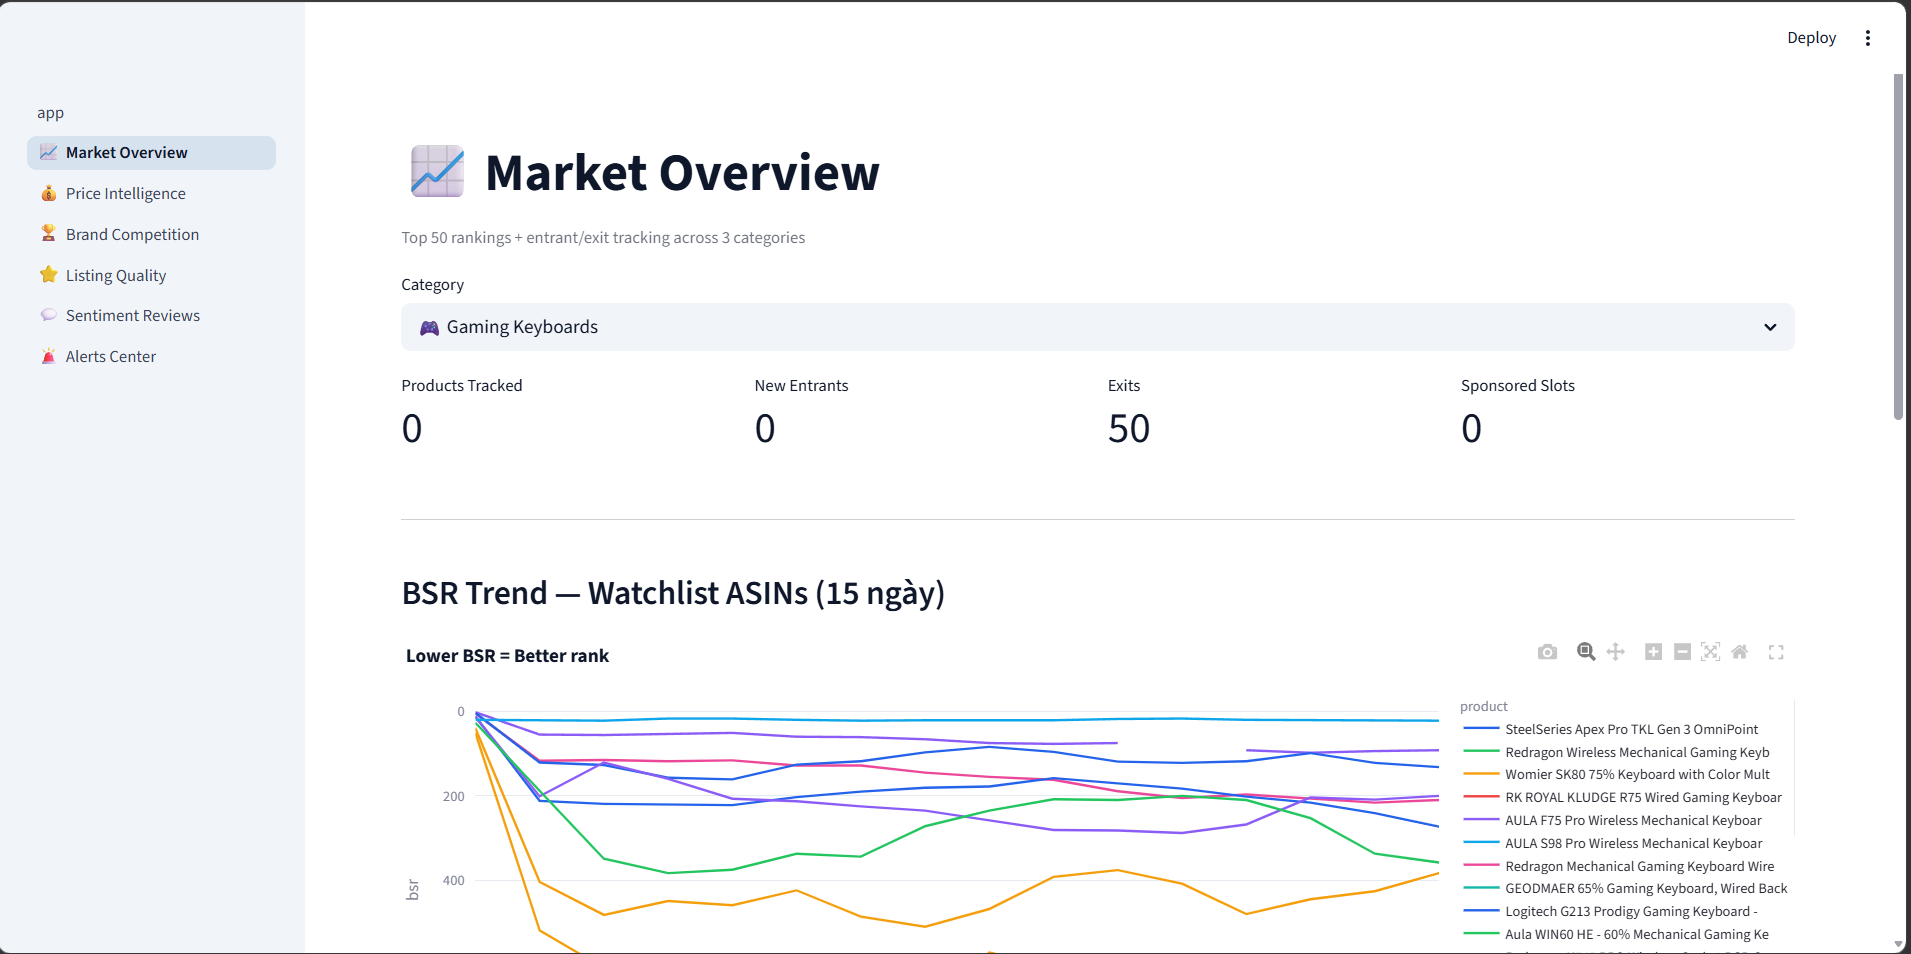
\includegraphics[width=\textwidth]{figures/dashboard_streamlit_overview.png}
  \caption{Streamlit dashboard overview showing the Market Overview page with category selector, summary metrics, and a BSR trend chart for watchlist ASINs. The sidebar lists the six analytical pages implemented under \texttt{dashboard/}. This interface supports pull-based exploration of the same Supabase tables that the OpenClaw agents query through read-only skills.}
  \label{fig:app_streamlit_overview}
\end{figure}

\begin{figure}[H]
  \centering
  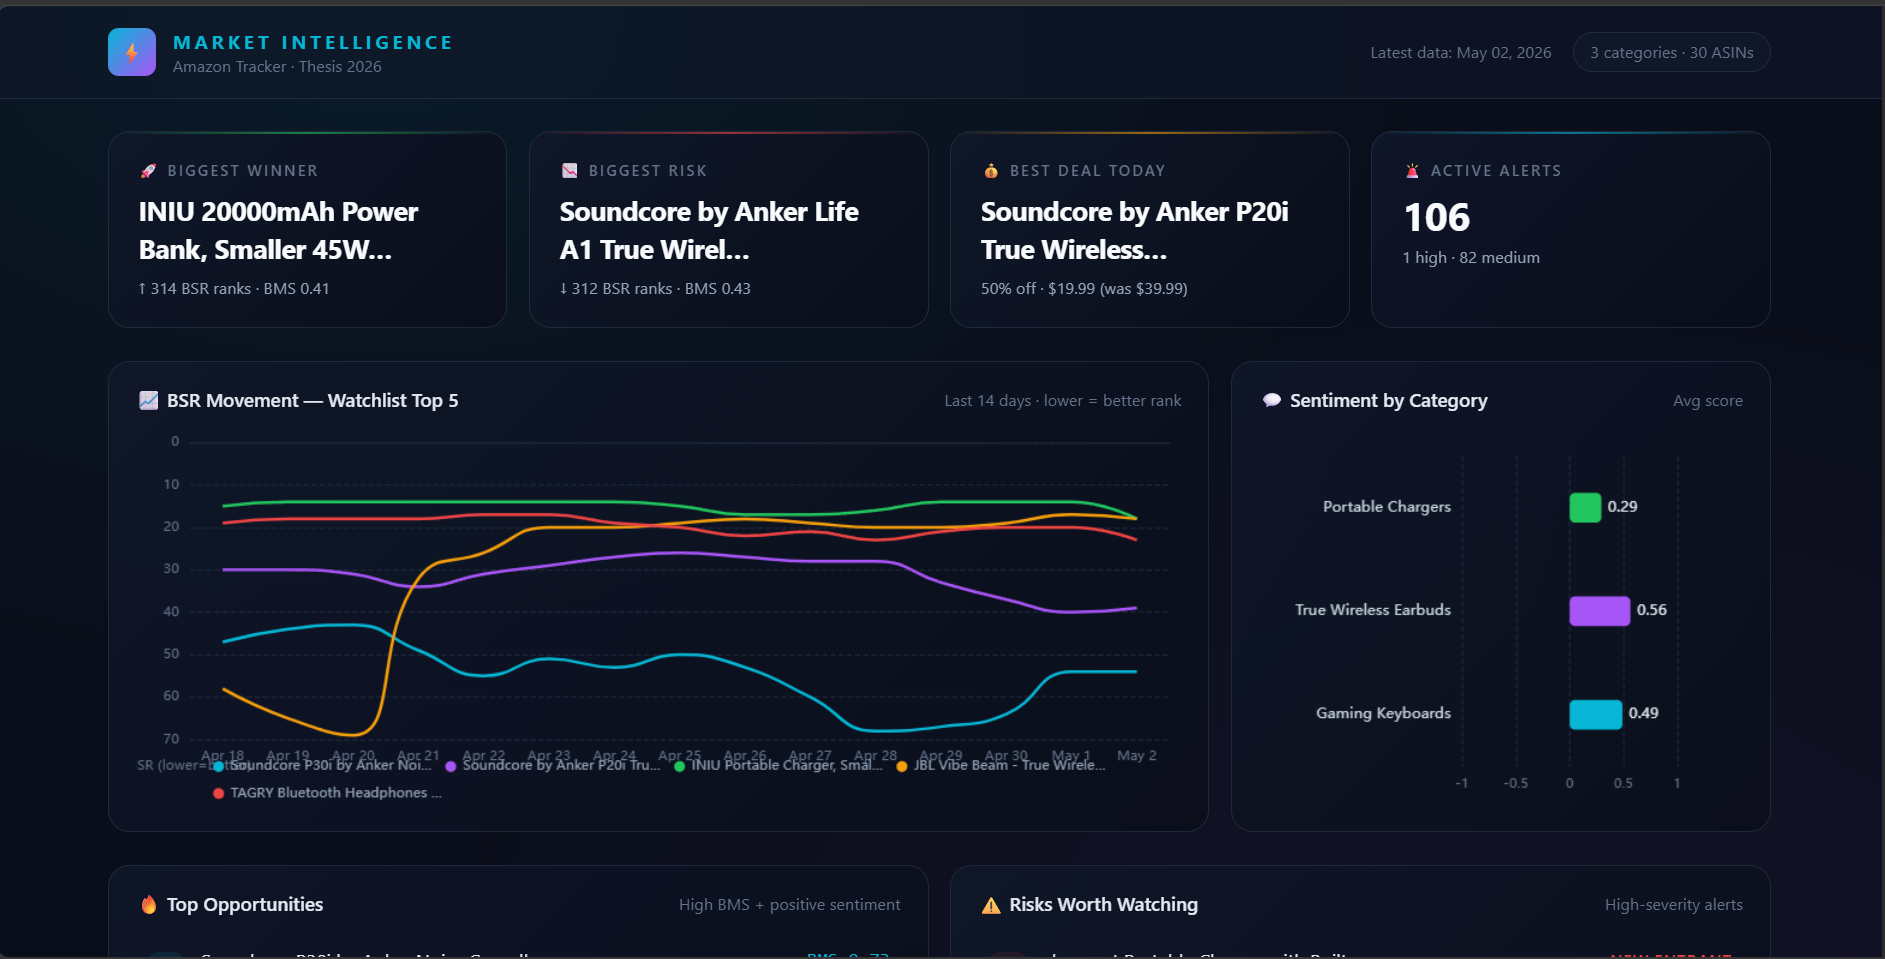
\includegraphics[width=\textwidth]{figures/dashboard_web_overview.png}
  \caption{Static web dashboard providing a compact market-intelligence overview backed by Supabase data. The interface displays key watchlist signals including top BMS movers, high-risk ASINs, active deal alerts, BSR movement trends, and category-level sentiment composition. This lightweight dashboard is deployable to Vercel and is designed for quick visual inspection rather than deep analytical exploration.}
  \label{fig:app_web_overview}
\end{figure}
